% !TEX program = lualatex
\documentclass{article}
\usepackage{fontspec}
\usepackage{luatexja-fontspec}
\usepackage{luatexja-ruby} % ルビを使用する場合に必要
\usepackage{graphicx}

% フォントの設定
%\setmainfont{Noto Serif JP}    % 通常の明朝体
%\setsansfont{Noto Sans JP}     % 通常のゴシック体
%\setmonofont{Noto Sans Mono JP} % 等幅フォント
%\setmainjfont{Noto Serif JP}   % 日本語の明朝体
%\setsansjfont{Noto Sans JP}    % 日本語のゴシック体
%\setmonojfont{Noto Sans Mono JP} % 日本語の等幅フォント

\graphicspath{{./01_code/output/}}

\begin{document}

% タイトル
\title{ミクロデータサイエンス\\Problemset1}
\author{2125178\\廣江友哉}
\date{\today}
\maketitle


% 段落
\section{サイコロと一様分布}

\subsection{分布の形}

どの実現値においても同じ確率 1/6 を取る長方形のような形の分布になる。

\subsection{コードの実行結果の考察}
	\begin{center}
		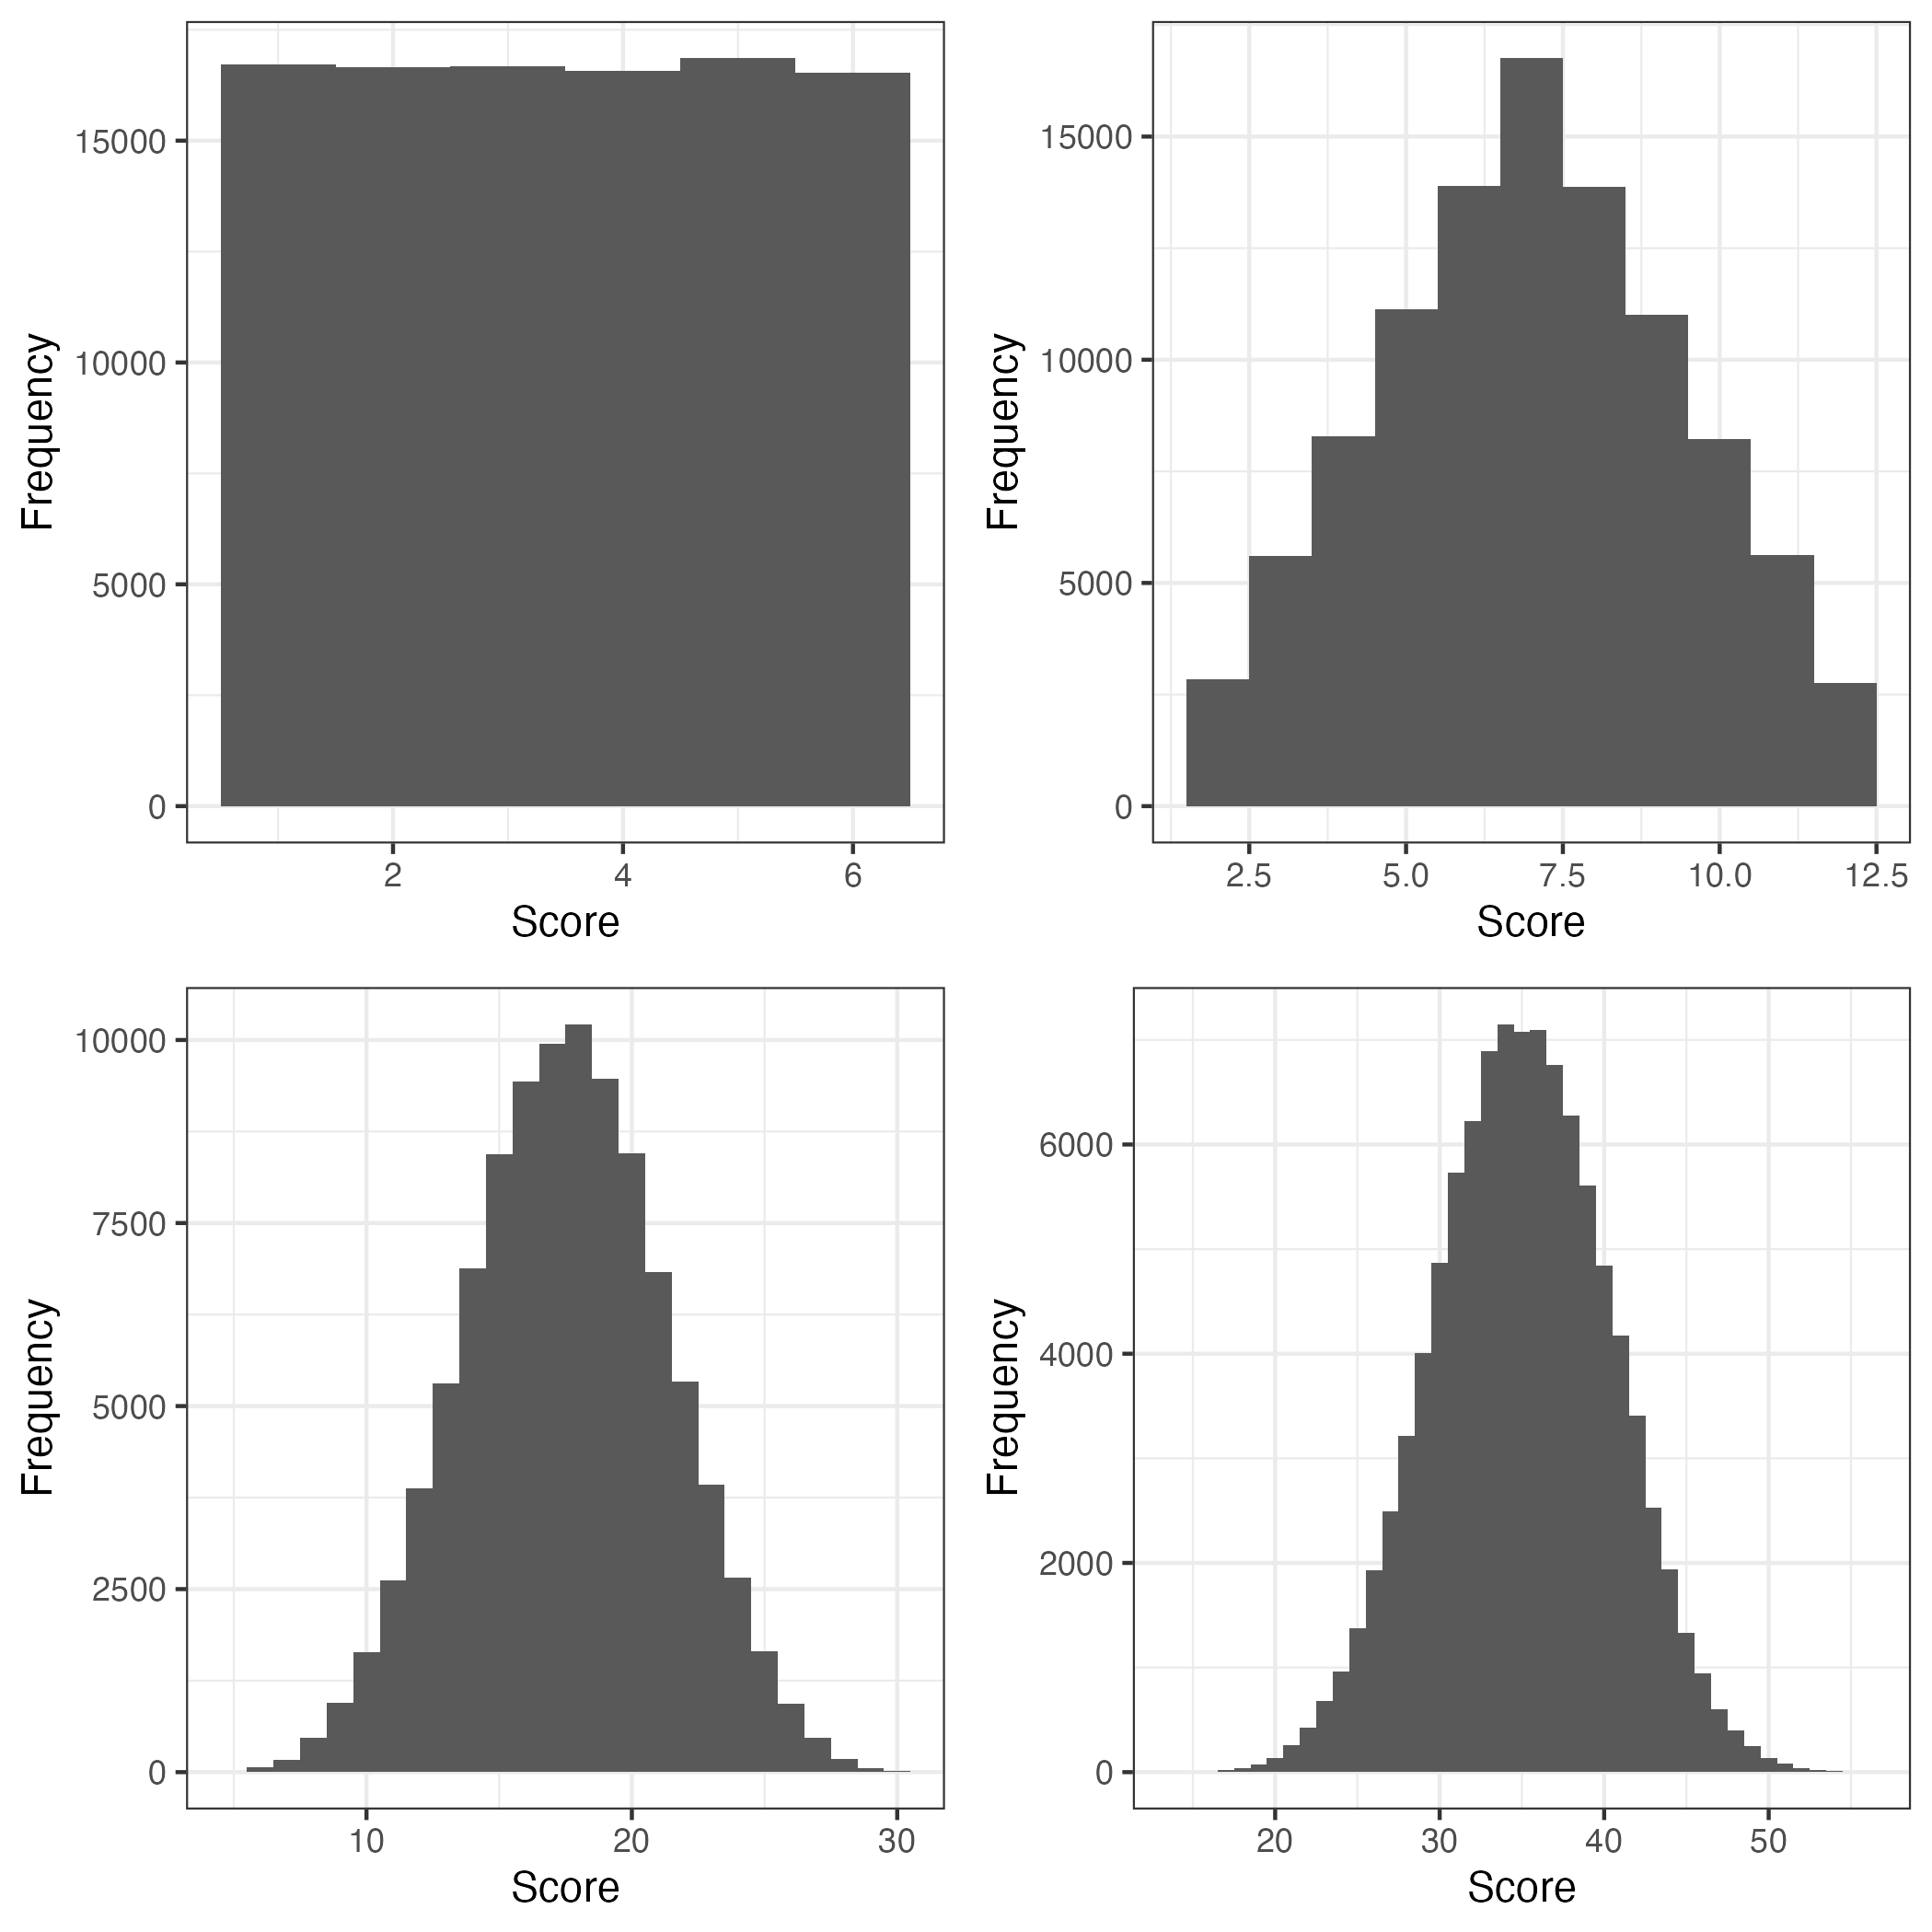
\includegraphics[width=0.7\textwidth]{1-2_plot.png}
	\end{center}

上図は、左上から順に、m = 1,2,5,10 の時の分布である。 
m = 1 の時は 1-1 で回答したように一様分布に従っている。\\
m = 2 から m = 10 にかけて少しずつ正規分布に近似していくのが見て取れる。\\
ここから、一様分布に従う確率変数の和は繰り返すと正規分布に近似することが考察できる。

\subsection{確率分布の和の分布のシミュレーションadv}

\subsection{標本平均の分散の変化}







\end{document}
